%\section{Задача реконструкции при зондировании полихроматическим излучением}

\begingroup
\small
\begin{frame}
\frametitle{Модель измерений}

При переходе к немонохроматическому случаю, уравнение затухания прошедшей через объект интенсивности: 
\begin{equation}
\notag
I(\varphi, \xi) = \int_0^{+\infty}{\left\{
  I_0(\lambda) \exp{\left(- {\mathrm R}[f(\lambda)](\varphi, \xi) \right)} d\lambda
  \right\}}  
\end{equation}


Будем считать, что объект состоит из $K$ элементов, с неизвестными пространственными концентрациями $c_k(x,y)$, и известными табулированными массовыми коэффициентами ослабления $\kappa_k(\lambda)$.
Тогда
$$
f(x,y, \lambda) = \sum_{k = 1} ^K {c_k(x,y) * \kappa_k(\lambda)}
$$

и прямая проекция для пикселя $j$ принимает вид

\begin{equation} \notag
  \label{eq:white_fp_final}
  I(c)_j = \int_0^{+\infty} {d\lambda \left\{
    I_0(\lambda) \exp{\left(
      -\sum_{k=1}^K {\rho \kappa_k(\lambda) (W c_k)_j} 
      \right)}
  \right\}}
\end{equation}

\end{frame}
\endgroup

\begin{frame}
\frametitle{Оптимизационная задача}

Следуя алгебраическому подходу, реконструкция проводится с помощью градиентного спуска оптимизации квадратичной функции потерь 
$$
Q(c) = \frac {\left(I(c) - t\right)^2} {S} \to \min \limits_c,
$$
где $t$ --- измеренные интенсивности прошедшего через объект излучения, \\
$S = \int_0^{+\infty} { I_0(\lambda) d\lambda}$
 --- суммарная интенсивность зондирующего излучения.

\end{frame}

\begin{frame}
\frametitle{Градиент функции потерь}
\begin{equation} \notag
\label{eq:part3_whitegrad}
  \nabla_k \ Q = 2W^\intercal R_k \text{, где } R_{kj} = \frac {(I(c) - t)_j} {S} \mu_{kj}
\end{equation}

а формулы для вычисления весов невязок по каждому элементу приведены ниже:
\begin{equation} \notag
  \label{eq:weights}
  \mu_{k} = \int_0^{+\infty} {d\lambda \left\{
    -\rho \kappa_k(\lambda) 
    I_0(\lambda)
    \exp{\left(
      -\sum_{s=1}^K {\rho \kappa_s(\lambda) (W c_s)} 
         \right)}
    \right\}}
\end{equation}

\end{frame}


\begin{frame}
\frametitle{Метод взвешенных невязок}
\framesubtitle{регуляризация}
  \begin{block}{Мультипликативная регуляризация}
    Запрещаем одновременное нахождение разных элементов в одном пикселе, т.е. $c_{k} \odot c_{s} = 0 \mbox{, если} k \neq s$.

    $$
    Q(c) + \beta\sum_{k_1 != k_2}\Norm{c_{k_1} \odot c_{k_2}} \to \min \limits_c
    $$
  \end{block}
  \begin{block}{Ограничение на значения концентраций}
  Используя метод барьерных функций, можем учесть, что концентрации имеют значения на интервале $[0, 1]$
    $$
    \begin{array}{lc}
    Q(c) \to \min \limits_c & w.r.t \\
    c_k \geq 0 & \\
    c_k \leq 1
    \end{array}
    $$
  \end{block}
\end{frame}

\begin{frame}
\frametitle{Исходные данные}
\begin{figure}
\centering
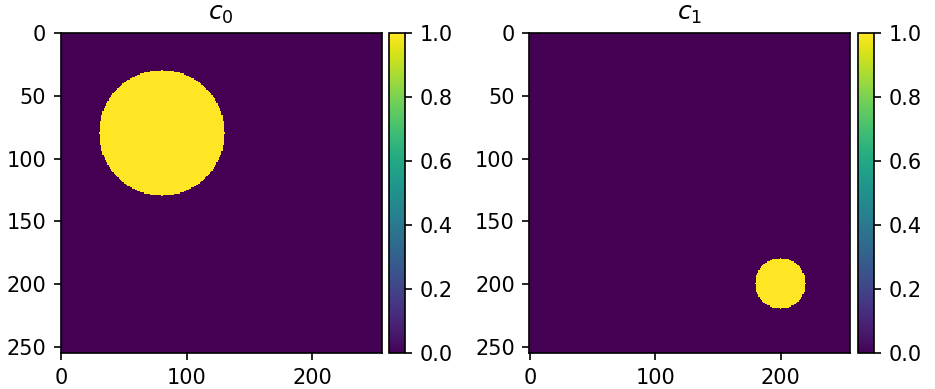
\includegraphics[width=\textwidth]{0999}
\\
\caption{фантом на тривиальных спектрах}
\end{figure}
\end{frame}


\begin{frame}
\frametitle{Исходные данные}
\begin{figure}

\centering
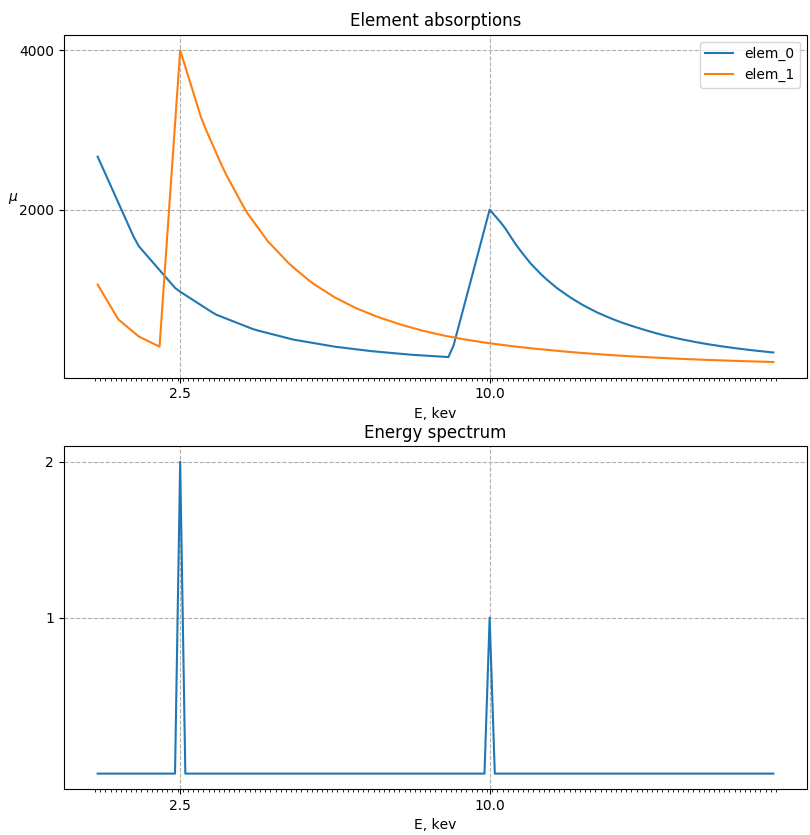
\includegraphics[height=0.7\textheight]{../Dissertation/images/part3_img/synth_spectre}
\\
\caption{спектры и массовые коэффициенты ослабления элементов}
\end{figure}

\end{frame}

\begin{frame}
\frametitle{Результаты восстановления}
\begin{figure}
\centering
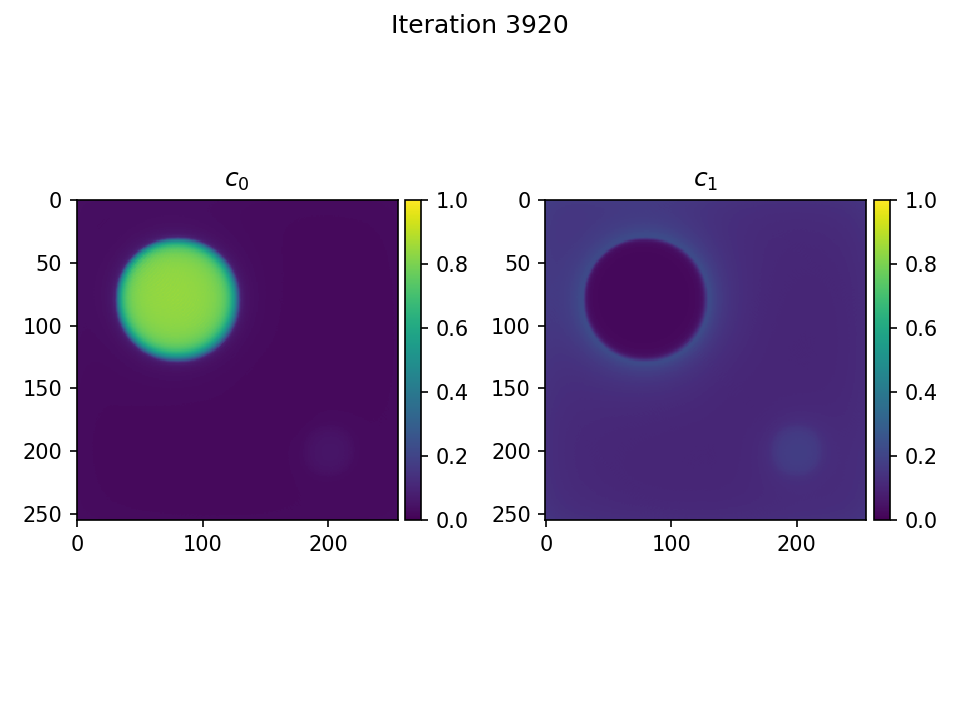
\includegraphics[width=\textwidth]{whiterec_res}
\\
\caption{Метод взвешенных невязок + метод барьерных функуий + мультипликативная регуляризация}
\end{figure}
\end{frame}